\documentclass[letterpaper]{article}
\usepackage{natbib,alifexi}
\usepackage[utf8]{inputenc}
\usepackage[english]{babel}
\usepackage{graphicx}
\usepackage{hyperref}
\usepackage{float}
\usepackage[colorinlistoftodos,prependcaption,textsize=tiny]{todonotes}


\title{Reinforcement learning approaches to movies recommendation}
\author{Antoine Carpentier$^{1}$, Pierre Gérard$^{2}$ \and Julian Schembri$^2$ \\
\mbox{}\\
$^1$Vrije Universiteit Brussel, Brussels \\
$^2$Université libre de Bruxelles, Brussels \\
antoine.carpentier@vub.ac.be, pierre.gerard@ulb.ac.be, julian.schembri@ulb.ac.be}


\begin{document}
\maketitle

\begin{abstract}
  The purpose of our research is to study reinforcement learning approaches to building a movie recommender system. We formulate the problem of interactive recommendation as a contextual multi-armed bandit, learning user preferences recommanding new movies and receiving their ratings. We show that using reinforcement learning solves the problem of exploitation-exploration tradeoff and the cold-start problem. We integrate the novelty of movies to the model. We explore a content based approach as well as a collaborative filtering approach and both yield viable recommendation results.
\end{abstract}

\section{Introduction}


People sometimes have to settle on decisions without sufficient individual experience of the choices. In regular daily existence, we depend on  recommendations from other individuals either by listening in conversations or by direct suggestion of movies, tv show, holiday destination, etc. Recommender systems help and enlarge this normal social process. 

In a recommender system, individuals usually give behaviour information as data sources, which the system then use to learn users preferences in order to provide recommendation. The recommender's value lies in its capacity to make great matches between the recommenders and those looking for suggestions. Such systems are the strength of content providers such Netflix \cite{netflix-article-recommender} or YouTube \footnote{http://www.youtube.com} allowing them to make their content more attractive in order to increase viewing and in order to optimise its monetisation. It allows to infer customer's center of interest and also allows to detect, if a behaviour is a general trend between customers, potential improvements in content to better meet the expectations of the public. 


This work follows the steps of \cite{main} who have implemented a music recommendation system using q-learning. In their research, \cite{main} explains was could be done to adapt their work to movies recommendation as well as a suggestion trying a collaborative filtering. So this work, is mainly about adapting their strategy of music recommendation to movies recommendation as well as exploring new strategies.

The problem of movie recommendation is modelised as a multi-armed bandit [\cite{sutton1998reinforcement}] thus allowing it to have the following advantages. 

\begin{itemize}
	\item The learning is done by incorporating user feedback (i.e. ratings of movies) into recommendations allowing us to fit diversity in users preferences,
	\item The model takes into account novelty of movies and repetitions thus not recommending movies watched recently,
	\item The learning balances exploration and exploitation thus mitigating the difficulty of cold-start,
	\item The model can take into account both a content based approaches and a collaborative filtering approaches.
\end{itemize}


In the following sections, we will firstly introduce methods used. Then we will review different results before discussing them.

\section{Methods}

\subsection{Data mining}

The data used is originated from IMDb \footnote{http://www.imdb.com/}. It is twofolds, the first part is a movie catalog containing relevant information about each movies such as the genre, keywords describing the content, the year, the rating by others users and votes count. That part is publicly available from IMDb FTP in a homemade format. The second part of data is RSS flux of movies watched and rated by IMDb users containing the title of the movie along the rating and the time it was watched.

\subsection{Features extraction and selection}

The first challenges was to extract the feature from the IMDb homemade format and made into a clearer \textit{csv} format.

In order to reduce the complexity of the algorithm and focus on the learning matter and not transforming the problem into a big data and parallelisation problem problem, a subset of movie, a selection of user and movies adding up to about 430.000 user-movie pair have been made.

Then for each movie and to also keep the problem simple and focus on the learning matter, we selected genre and year as features for each movie. Those two features are categorical variable and in order to learn a single weight per feature (i.e. drama, crime, ..), a onehot encoding have been apply to them resulting in a blow up of the feature space to $n$ features, $n$ being the number of category.

\begin{table}[h]
\center{
\begin{tabular}{|c|c|c|c|c|}\hline
 Name       & Drama & Crime & Thriller & ... \\ \hline
Movie 1  & 0   & 0 & 1 & ...\\ \hline
Movie 2  & 1 & 1 & 1 & ...\\ \hline
Movie 3  & 0 &   0 & 0 & ...\\ \hline
... & ... & ... &  ...  &  ... \\ \hline
\end{tabular}
}
\vskip 0.25cm
\caption{Movies feature space}
\end{table}


\subsection{Dimension reduction}

The resulting feature space of the feature extraction process is quite sizable thus making the recommendation quite computational intensive.
In order to deal with that problem, the feature space size has been reduced using Principal Components Analysis (PCA) [\cite{principalcompanalysis}].

The principal components analysis is a machine learning procedure that apply an  orthogonal transformation to the dataset in order to obtains a new set of values which have the property of a minimised covariance. Those new variables are called principal components. There are ordered in term of variance, the first principal component having the highest variance and so on. When the procedure is applied a reduction to n-dimension consists of keeping the n-first principal components.

For our dataset we kept, the 20-first principal components out of about 50, keeping about 83\% of the variance of the original dataset.

\begin{figure}[H]
\begin{center}
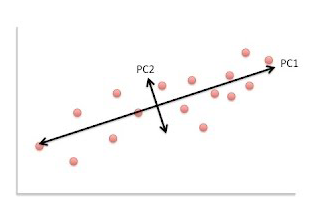
\includegraphics[width=2.1in]{img/pca.png}
\caption{Example of a 2 dimension PCA. A reduction to one dimension would be to keep only PC1.}
\label{pca}
\end{center}
\end{figure}

\subsection{Multi armed bandit modelling}

The multi-armed bandit is a intensively studied reinforcement learning dilemma. It consists of a bandit (usually a casino slot machine) with $K$ arms, each giving a payoff $r$ sampled from an unknown probability distribution $p_{i}$. The player has a defined $n$ number of pulls and its goal is to choose wisely which arm to play in order to maximise the total payoff.

The movie recommendation problem can be seen as a bandit problem where each arm is a movie and a user can pull it (watch it). The reward or loss or can be seen as the difference between the expected rating of a movie for a suer and the the true rating given as a feedback by the user. As the number of arm is gigantic and each arm are not even played once, an heuristic is used to help the system into choosing an arm. The heuristic can be content based or a collaborative filtering.

\begin{figure}[H]
\begin{center}
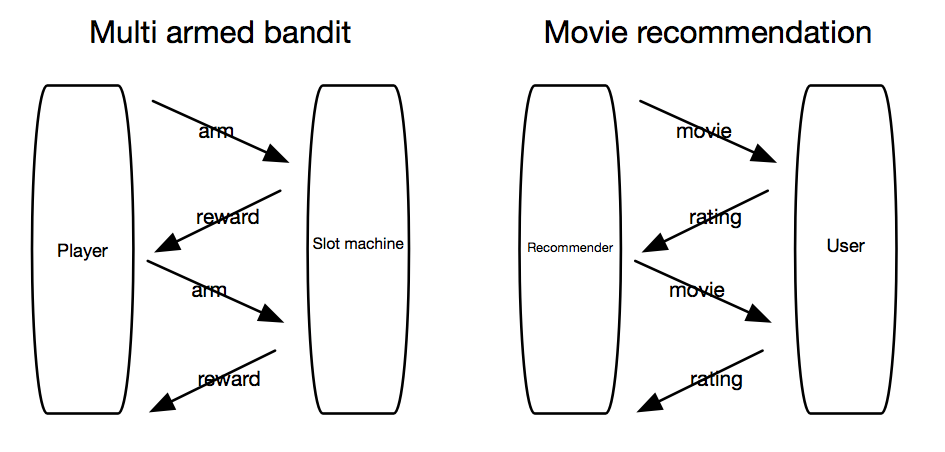
\includegraphics[width=3.4in]{img/schema.png}
\caption{Seeing a movie recommender as a multi-armed bandit problem}
\label{schema}
\end{center}
\end{figure}

\subsubsection{Content based}

The content based heuristic try to find a movie that is close to the learned user preferences $\theta$. It takes into account the movie genre, movie year and novelty. Novelty can be defined as if the movie as been recently watched or not.

The movie genre and movie year can be considered as a onehot encoded vector $x$.
Without considering other factor, the utility of a user for a movie can be represented as the following.

\begin{center}
	$ \ U_{c} = \theta^{T} * x$ 
\end{center}

Distinctive users have different preferences $\theta$. Also, we do the hypothesis of a stationary true value for $\theta$, meaning that while, we learn the user preference, its preferences stay the same.

The novelty is defined using the forgetting curve proposed by \cite{ebbinghaus1913memory} and defined as $ e^{\frac{t}{s}} $ with $t$ being the current time and $s$ an hyper-parameter defining how fast we forget and want a repetition. Obviously for movie an higher value of $s$ is needed compared to an $s$ that would be used for music. The utility for a user in term of novelty can be defined as follows.

\begin{center}
	$ \ U_{n} = 1 - e^{\frac{t}{s}} $ 
\end{center}

The combined utility or more explicitly the expected rating for a movie and a user is defined as follows.

\begin{center}
	$ \ U = \ U_{c} *  U_{n} = (\theta^{T} * x) * (1 - e^{\frac{t}{s}}) $ 
\end{center}

The last task of the recommender is then to propose the movie with the highest expected rating to the user and update the user preferences $\theta$ according to the difference in rating received and predicted.

\subsubsection{Collaborative filtering}

The collaborative filtering heuristic try to find a movie that is a liked movie by a similar user. It takes into account others users rating and novelty of a movie.

The algorithm will start by finding a cluster of the user and $k$ others users by associating of the most similar user in clusters. The association is done by calculating the Pearson product-moment correlation coefficient on preferences $\theta$ of the targeted user and others users. Then cluster users rating are considerate to be the utility of the user for those movie. In others words, similar user's movies rating become targeted user utility for those movies.

\begin{center}
	$ \ U_{f} = u $ 
\end{center}

Note that others users rating are weighted by the average means they give to movie to avoid biais.

The novelty if defined similarly as above, so the expected rating is :

\begin{center}
	$ \ U = \ U_{f} *  U_{n} = u * (1 - e^{\frac{t}{s}}) $ 
\end{center}



\subsection{Bandit strategies}

Many strategy to find an approximate solution have been developed over the years. A review of them is explain by \cite{kuleshov2014algorithms}.

\subsubsection{Random}

The random strategy is not a real strategy per se. It is a strategy where the player will only do exploration. It is mostly used as a basis to compare the effectiveness in term of reward or regret of an other algorithm.

\subsubsection{Greedy-epsilon}

The $\epsilon-greedy$ algorithm is widely used because it is fairly simple. For each round of the simulation, the algorithm selects the arm (movie) with the highest expected value based on the context vector with a probability of $1-\epsilon$ and selects a random arm with a probability $\epsilon$.

\subsubsection{Greedy time dependent}

The greedy time dependent is a variation of the previously mentioned greedy where $\epsilon$ variated over time in order to maximise the exploration at first and reduce it in order to increase exploitation over time.

\begin{center}
	$\epsilon = \frac{1}{\sqrt{t+1}}$
\end{center}

However, the effectiveness of variating $\epsilon$ over time is disputed by \cite{vermorel2005multi} whose did not find any practical advantage to using these method. As a result, we will test both approaches.

\subsubsection{Greedy UCB}

\todo{GreedyUCB}

\subsubsection{Bayes UCB}

\todo{BayesUCB}
% """Priors for the Bayesian models were set as uninformative ones or chosen based on preliminary sim- ulation and user studies""" < ce qui notre tache très difficile

\subsubsection{Bayes inference}

\todo{Bayes inference}

\subsection{Simulation}

We conducted an empirical efficiency study of the algorithms mentioned above as well as the content based and collaborative filtering modeling. 

Experiments were conducted on personal computer and the programming language $python$ was used to implement models and algorithms.

The simulation consisted on simulating the interaction of a user and a recommender. \todo{explain the simulation better}


% ------ results -------
\section{Results}

\todo{simple result of adaptation of music paper to movie paper avec greedy vs random}

\todo{more diverse choice in bandit strategies including}

\todo{result of collaborative filtering}


% ------ discussion -------
\section{Discussion}

\todo{would the result be correct recommendation, is it a viable way to do recommendation ? (expected result vs reality, time for a recommendation, accuracy, ....)}

\todo{which strategy to use and which not to use ( including why bayes-ucb is not viable (way too much time an requires a user study to bootstrap)}

\todo{content based vs collaborative, is collaborative viable}

\todo{futur work, what could be done if you give me 10 IA guys for a week}

\section{Conclusion}

blabla

\footnotesize
\bibliographystyle{apalike}
\bibliography{biblio}


\end{document}


%\begin{figure}[t]
%\begin{center}
%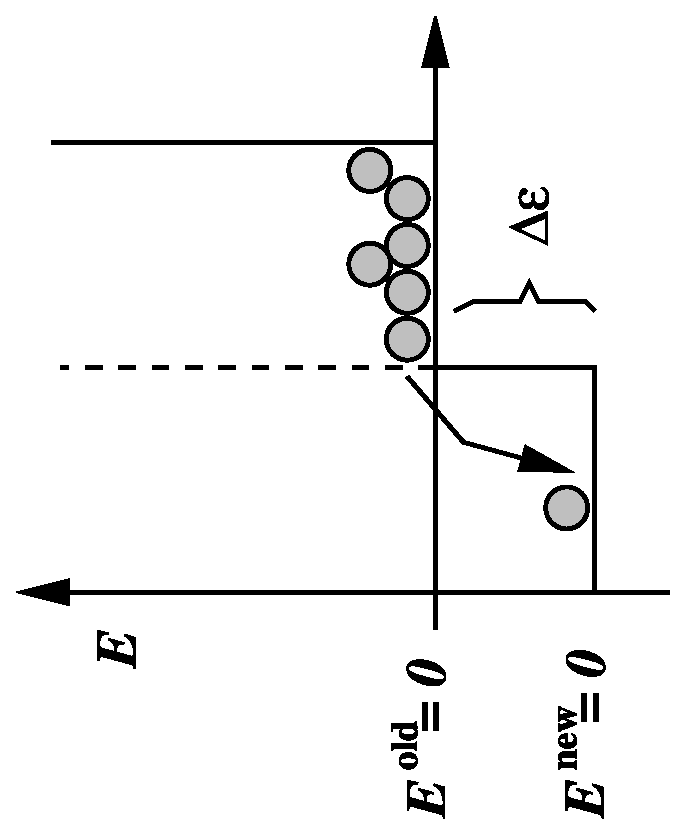
\includegraphics[width=2.1in,angle=-90]{img/fig1.eps}
%\caption{``Energies'' (inferiorities) of strings in a first-order
%  phase transition with latent heat $\Delta\epsilon$.}
%\label{fig1}
%\end{center}
%\end{figure}
